\documentclass[crop,tikz]{standalone}
\usepackage[T1]{fontenc}
\usepackage{tikz}
\usetikzlibrary{matrix,backgrounds,arrows.meta,fit,positioning,decorations.pathreplacing}
\begin{document}

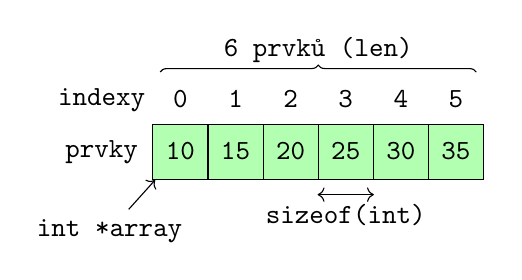
\begin{tikzpicture}[font=\ttfamily,
  array/.style={matrix of nodes,nodes={draw, fill=green!30,minimum size=7mm},column sep=-\pgflinewidth, row sep=0.5mm, nodes in empty cells,text height=1.5ex, text depth=.25ex,
    row 1/.style={nodes={draw=none, fill=none, minimum size=5mm}},
}]

\matrix[array] (array) {
 0 & 1 & 2 & 3 & 4 & 5 \\
  10 & 15 & 20 & 25 & 30 & 35 \\ };

\draw[decoration={brace},decorate]([yshift=+1mm]array-1-1.north west) -- node[above] {6 prvků (len)} ([yshift=+1mm]array-1-6.north east);

\draw[<->]([yshift=-9mm]array-2-4.north west) -- node[below] {sizeof(int)} ([yshift=-9mm]array-2-4.north east);

\node[left of=array-1-1] {indexy};
\node[left of=array-2-1] {prvky};

\draw[->] node[below of=array-2-1,xshift=-9mm] {int *array} edge (array-2-1);

%\draw[<->] (array-2-1.south) edge [bend right] (array-2-5.south);
%\draw[<->] (array-2-2.south) edge [bend right] (array-2-4.south);

\end{tikzpicture}
\end{document}
